\chapter{Hasonló megoldások vizsgálata}
\label{cha:related_work}

Mielőtt a saját Wikipédia alapú rendszer tervezésének nekiláttam volna megvizsgáltam a hasonló célú, elérhető megoldásokat, hogy utána a tapasztalatokból kiindulva láthassak neki a munkának. Megpróbáltam összegyűjteni az összes hasonló témakört feldolgozó alkalmazást, majd ezeket egyesével megvizsgáltam, milyen előnyökkel, hátrányokkal rendelkeznek.

\begin{description}
	\item[WikiNet \cite{wikinet}] A WikiNet egy teljesen struktúrált adatszerkezetű tudásbázist, más néven ontológiát épít fel. Ez egy Perl nyelvű szkriptek gyűjteményéből álló megoldás, a Wikipédia egy statikus, letöltött verzióját használja forrásként, a kinyert fogalmakat és kapcsolatokat külön szöveges fájlokban tárolja el.
	
\textit{Elérhetőség:}\\
\url{http://www.h-its.org/english/research/nlp/download/wikinet.php}

	\item[DBpedia] Ez a megoldás is a Wikipédia dump-ján alapul, belőle tényszerű információkat nyer ki és rögzít struktúrált formában, melyet ezután a weben közzétéve a felhasználók számára egy SQL szerű nyelvvel lekérdezhetővé tesz. A alkalmazás Scala, Java nyelven íródott, adatbázisként Virtuoso Universal Server-t használ.
	
\textit{Elérhetőség:}\\
\url{http://dbpedia.org/}

\item[BabelNet \cite{babelnet}] A BabelNet egy Java nyelven írt alkalmazás, ontológiát készít más adatforrások (Wikipédia dump, WordNet) alapján és ezekből egy ``enciklopédikus szótárat'' készít a felhasználók számára. Egy adott fogalomra keresve a szemantikailag kapcsolódó fogalmak is megjelennek, valamint ezek szinonimái (a BabelNet elnevezése szerint \textit{synset}-ek), és minden szinonimához tartozik egy rövid definíció (\textit{gloss}) több nyelven.
	
\textit{Elérhetőség:}\\
\url{http://lcl.uniroma1.it/babelnet/}

\item[Java Wikipedia Library \cite{jwpl}] A JWPL egy Java alapú alkalmazás, mely egy interfészt ajánl ki, amivel a Wikipédia tartalmához lehet hozzáférni. A JWPL tartalmaz egy Mediawiki Markup parser-t, mellyel a letöltött Wikipédia dump-ot beolvassák, a wikitext-ből átalakított szövegekből optimalizált adatbázisokat készítenek, melyekhez végül hozzáférési felületet nyújtanak.
	
\textit{Elérhetőség:}\\
\url{http://www.ukp.tu-darmstadt.de/software/jwpl/}

\item[Wikipedia Preprocessor] Ezzel az eszközzel más alkalmazások számára lehet egy Wikipédia dump-ot feldolgozhatóbb formába hozni. A statikus dump-ból kiinduló alkalmazásoknál erre szükség is van, mivel a például Wikipédia 2013. október 2-i XML formátumban letölthető tartalma is 44 GB méretű, amit nyers formában szinte lehetetlen hatékonyan felhasználni.
	
\textit{Elérhetőség:}\\
\url{http://www.cs.technion.ac.il/~gabr/resources/code/wikiprep/}

\item[YAGO2 \cite{yago2}] A YAGO2 a Wikipédia egy korábban letöltött tartalmán, és egyéb online tudásbázisokon (WordNet, GeoNames) alapuló ontológia. Az ontológiához több formátumban lehet hozzáférni, ezt kisebb Java nyelven írt konvertáló eszközökkel lehet megtenni.
	
\textit{Elérhetőség:}\\
\url{http://www.mpi-inf.mpg.de/yago-naga/yago/}
\end{description}

\section{Egy ígéretes megoldás: Wikipedia Miner}
\label{sec:wikipediaminer}

A Wikipedia Miner egy olyan nyílt forráskódú teljes egészében Java nyelven írt eszközkészlet, mellyel lehetővé válik kutatók és fejlesztők számára, hogy alkalmazásukban egyszerűen hozzáférjenek a Wikipédia tartalmához. A hozzáférési felületet Java API-n keresztül nyújtja az alkalmazás, a tudásbázis tartalmát pedig egy összegzett formában használja fel. Ezenfelül a rendszer olyan technológiákat használ fel, mint az elosztott számítási keretrendszert nyújtó Apache Hadoop és a Weka adatbányászati szoftver.

A Wikipedia Miner alkotói szerint három lehetőség van a szemi-struktúrált adatforrások felhasználására: vagy kész ontológiákat használunk, mint például a YAGO2, vagy egy nyers letöltött dump-ból elkészítjük a saját ontológiánkat, mint például a JWPL és az alapján kezdünk dolgozni; a harmadik lehetőség, hogy folyamatosan frissítjük az adatforrásunkat, így mindig naprakész forrást használunk.

\begin{figure}[htp]
\centering
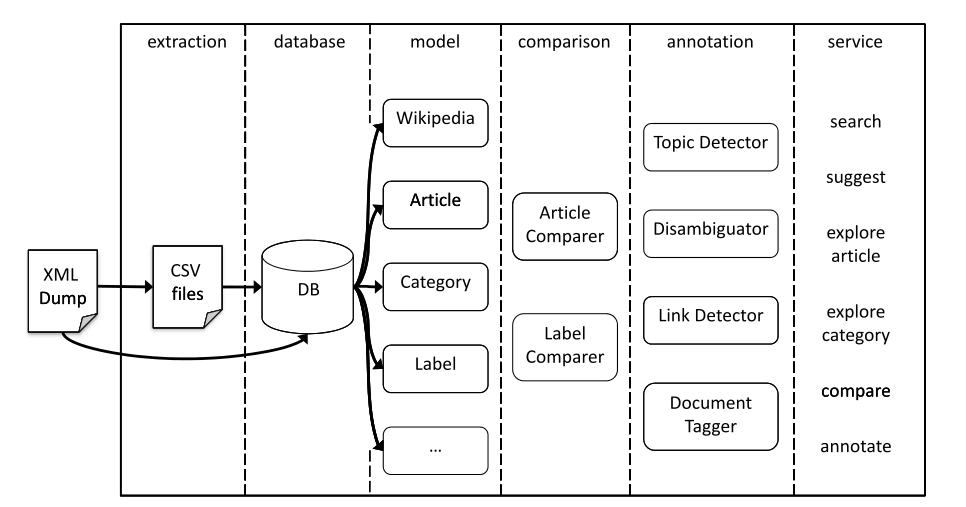
\includegraphics[scale=0.4]{img/wikipediaminer}
\caption{Wikipedia Miner architektúra (forrás: Artificial Intelligence, Wikipedia and Semi-Structured Resources \cite{aijournal})}
\label{fig:wikipediaminer}
\end{figure}

A rendszer áttekintő architektúráját mutatja be a \ref{fig:wikipediaminer}.~ábra. A rendszer belépési pontjára érkezik egy nagy méretű XML formátumú fájl, mely a Wikipédia hivatalos API-ján keresztül lett letöltve és tartalmazza a naprakész Wikipédia teljes állományát.

Az \textit{extraction} package funkciója, hogy kinyerjen az XML forrásból egy összegzett tartalmat. Az adatkinyerési folyamat használja a nagy méretű XML fájl feldolgozásához a Hadoop és MapReduce technológiákat, valamint a Google GFS fájlrendszerét. Az adatok kinyerése tehát elosztott rendszeren történik, a 27 GB méretű teljes angol Wikipédia feldolgozása a mérések szerint egy 2 magos, 2,66 GHz órajelű processzorral és 4 GB memóriával rendelkező 30 gépből álló clusternek 2,5 órájába telik.

A Wikipédia kivonatolása után a teljes XML fájl és az összegzett tartalmak is bekerülnek a \textit{database} package adatbázisába. Adatbázisként Berkeley DB Java Edition-t használnak, mellyel akár egy teljes adatbázist is a memóriában lehet tartani, ezzel nagyon gyors lekérdezhetőséget elérve.

A Wikipedia Miner keretrendszert használók a tartalmakhoz a \textit{model} package absztrakciós felületen keresztül férhetnek hozzá, mely becsomagolja a kinyert információkat és jól dokumentált osztályok formájában teszi közzé (mint például: \texttt{Wikpedia}, \texttt{Article}, \texttt{Category}).

A további csomagok (\textit{comparison} és \textit{annotation}) már a felhasználók számára használható szemantikus tartalom kezelését segítő eszközök, a \textit{service} package-ben pedig konkrét szolgáltatások találhatóak, melyeket felhasználhatnak a fejlesztők, illetve kiegészíthetik őket.

% section wikipediaminer (end)

\section{Tanulságok}
\label{sec:conclusion}

Amint látható a fentebb leírt Wikipédiát felhasználó eszközök szinte mind kizárólag a Wikipédia egy korábban letöltött változatán (dump) alapulnak, mely módszernek több hátránya is van. A letöltött tudásbázis mérete rendkívül nagy, így azt kezelni nehézkes, feldolgozási ideje rendkívül hosszú (a Wikipedia Processor feldolgozási ideje például körülbelül 43,5 óra). A hosszú feldolgozási idő nem mindig engedhető meg, ráadásul amíg nincs feldolgozott forrás, a rendszer sem működőképes. Újabb dump letöltésekor kezdhető előlről a feldolgozás, így többször is megakaszthatja ez a folyamat a rendszer működését, a rendelkezésre állási időt csökkentve.

A másik megoldás, melyet a Wikipedia Miner (\ref{sec:wikipediaminer}.~alfejezet) is demonstrál a Wikipédia folyamatos \textit{on-the-fly} feldolgozása. Míg az előző módszer figyelmen hagyja a közösségi tudásbázisok fő erejét, hogy rendkívül dinamikusan fejlődnek, az on-the-fly megoldás kihasználja azt, és mindig a friss adatokkal dolgozik.

További fontos megállapítások, hogy egyik rendszer sem elég flexibilis: futásidőben új komponens beépítése egyáltalán nem lehetséges, nem lehet a feldolgozólánchoz új elemet (kutatást végző modult) illeszteni, szerkezetük szinte mindegyiknek rendkívül statikus és csak arra a célra használhatóak konkrétan, amilyen speciális feladat ellátására kitalálták. Ebből adódóan rendkívül specifikusak és bonyolultak, így újabb kutatások indítása eredményeiket felhasználva nehézkes.

A szoftverek bármely módosítása újrafordítást, rendszerleállást eredményez, ami egy aktívan használt program számára nagy kiesést jelenthet. On-the-fly feldolgozásnál a rendszer leállása kihagyott, nem feldolgozott információkkal jár, így a tudásbázis töredezetté válhat. Ezen okok miatt szükséges egy olyan megoldás, mellyel a rendszer sokkal flexibilisebbé tehető és a fenti problémák áthidalhatóvá válnak.

% section conclusion (end)

% chapter related_work (end)